\documentclass{ximera}
\title{What is a system}

\maketitle

\begin{abstract}
This activity describes what is a system of ordinary differential equations.
\end{abstract}

\maketitle

\begin{sectionOutcomes}
After completing this section, students should be able to do the following:

\begin{itemize}
\item Recognize a system of ODEs.
\item Interpret a system of ODEs as a vector field.
\item Understand the representation of a vector field in the phase plane.
\end{itemize}

\end{sectionOutcomes}

To introduce the concept of a system of ODEs, let's consider the \emph{Lotka-Volterra predator-prey model}, which describes two animal species in the wild, traditionally referred to as ``rabbits'' (the prey) and ``foxes'' (the predator). Denoting by $R(t)$ and $F(t)$ the rabbit and fox populations, respectively, we use the following differential equations to model the dynamics of the two species in the wild:
\begin{align}
\label{rabbit-eq}R'&=aR-bRF\\
\label{fox-eq}F'&=cF+dRF
\end{align}
How do ecologists come up with this model? This is not a simple question, since there usually are many possible ways of modeling a real-world system. As a rule of thumb, scientists try to use the simplest possible model as a first approximation. For the predator prey model, the following are reasonable hypothesis:

%\begin{itemize}
%\item 
In the absence of predators, the prey population grows without limits. We can model this by an exponential growth model:
\[
R'=aR\text{ where $a>0$}.
\]
%\item 
In the absence of prey, the predator population decays to zero, since they don't have any available food. This can be modeled by an exponential decay model:
\[
F'=-cF\text{ where $b>0$.}
\]
%\item
To model the interactions between the two populations, we assume that the number of possible ``predation situations'' is proportional to the number of possible ``encounters'' between individuals of the two populations, which can be approximated by the product $RF$.
%\item 
Since predation is disadvantageous to the prey population, we subtract a term proportional to $RF$ to the prey equation:
\[
R'=aR-bRF\text{ where $a,c>0$}.
\]
%\item 
Since predation is beneficial to the predator population, we add a term proportional to $RF$ to the predator population:
\[
F'=-cF+dRF\text{ where $b,d>0$.}
\]
%\end{itemize}
Putting all together, we get the pair of equations~\ref{rabbit-eq},~\ref{fox-eq}.

\begin{problem}

Let's consider now consider two populations $x$ and $y$ that are in competition with each other. We make the following assumptions:
\begin{itemize}
\item In isolation, each of the populations grows exponentially. We denote the growth rates for $x$ and $y$ by $a>0$ and $c>0$, respectively. 
\item The effect of competition to each population is proportional to the product of the populations sizes, $xy$. We denote the corresponding proportionality constants for populations $x$ and $y$ by $b>0$ and $d>0$, respectively.
\end{itemize}

\begin{question}
$x'= \answer{ax-bxy}$
\end{question}
\begin{question}
$y'= \answer{cy-dxy}$
\end{question}
\end{problem}

%\begin{explanation} 
%In the absence of competition, the dynamics for each population is given by an exponential growth model:
%\begin{align*}
%x'&=ax\\
%y'&=cy.
%\end{align*}
%Competition has a negative effect on the growth of each population, so we need to subtract a term proportional to $xy$ to each equation, obtaining:
%\begin{align*}
%x'&=ax-bxy\\
%y'&=cy-dxy.
%\end{align*}
%\end{explanation}

\begin{problem}
A more realistic assumption in the predator-prey model is that the prey population grows logistically in the absence of predators. Write the system of ODEs for this situation, using $a$ for the intrinsic growth rate and $K$ for the carrying capacity of the rabbit population:
\begin{question}

$R'= \answer{ax(1-x/K)-bxy}$
\end{question}
\begin{question}

$F'= \answer{-cx+dxy}$
\end{question}
\end{problem}

\begin{problem} Another way in which system appear is in modeling higher-order differential equations. Recall the general equation for the unforced harmonic oscillator:
\[
mx''+cx'+kx=0,
\]
where $m>0$, $c\ge 0$ and $k>0$. The variable $x$ represents the displacement of the mass. Let $y$ represent the velocity of the mass. Write below a system of ODEs for the variables $x$, $y$:

\begin{question}
$x'= \answer{y}$
\end{question}

\begin{question}
$y'= \answer{-(k/m)x-(c/m)y}$
\end{question}

%\begin{explanation} The interpretation of derivative of displacement as velocity gives directly:
%\[
%x'=y.
%\]
%Plugging this into the equation of the harmonic oscillator yields:
%\[
%y'=x''=-\frac{k}{m}x-\frac{c}{m}x'=-\frac{k}{m}x-\frac{c}{m}y.
%\]
%\end{explanation}
\end{problem}

We now proceed to the numerical and graphical interpretation of a system of ODEs. Let's go back to the predator-prey model, this time assuming concrete values for the parameters $a$, $b$, $c$ and $d$:
\begin{align}
\label{rabbit-eq-c}R'&=1.2R-0.5RF\\
\label{fox-eq-c}F'&=-F+1.5RF
\end{align}
Since we have a concrete example now, it is advisable to set specific units for all variables. Let's assume that:
\begin{align*}
t&=\text{Time, measured in weeks;}\\
R&=\text{Rabbit population, measured in thousands of individuals;}\\
F&=\text{Fox population, measured in hundreds of individuals.}
\end{align*}
Notice that we use different units for the rabbit and fox populations, since the number of predators is usually much smaller that the number of prey in a realistic situation.

Next suppose that, at a certain time, we have the values:
\[
R=4,\quad F=3
\]
With this information, we can compute the rates at which each of the populations are growing, by plugging in the values of $R$ and $F$ into the equations~\ref{rabbit-eq-c} and~\ref{fox-eq-c}:
\begin{align*}
R'&=1.2\cdot 4 - 0.5\cdot 4\cdot 3=-1.2\\
F'&=-4 + 1.5\cdot 4\cdot 3=15.0
\end{align*}
In particular, we can conclude that, for these particular sizes of the rabbit and fox population, the number of rabbits is decreasing and the number of foxes is increasing.

\begin{problem} Suppose that at a certain time, the rabbit population is  $5000$ and the fox population is $100$. Find the rate of change of the populations, and determine if each population is increasing and decreasing.

\emph{Hint}: Notice that you will have to scale the populations in the appropriate way!

\begin{question}
$R'= \answer{3.5}$

The rabbit population is 
\begin{multipleChoice}
\choice[correct]{Increasing}
\choice{Decreasing}
\end{multipleChoice}
\end{question}
\begin{question}
$F'= \answer{6.5}$

The fox population is 
\begin{multipleChoice}
\choice[correct]{Increasing}
\choice{Decreasing}
\end{multipleChoice}
\end{question}
\end{problem}

We can also represent the rates of change geometrically. We interpret the pair of derivatives $(R',F')$ as the components of a vector:
\[
\begin{bmatrix}R'\\F'\end{bmatrix}=
\begin{bmatrix}1.2R-0.5RF\\-F+1.5RF\end{bmatrix}
\]
Then, for $R=4$ and $F=3$ we have:
\[
\begin{bmatrix}R'\\F'\end{bmatrix}=
\begin{bmatrix}-1.2\\15.0\end{bmatrix}
\]
This can be represented graphically as in the figure below:
\begin{center}
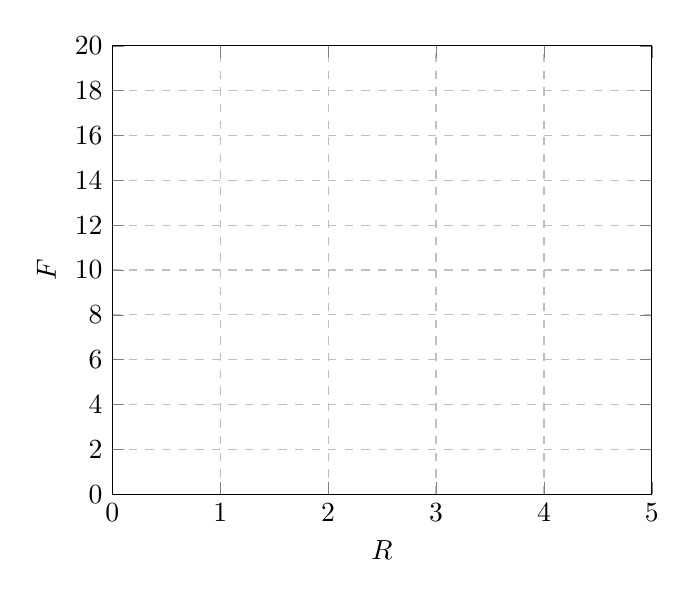
\begin{tikzpicture}
	\begin{axis} [
		xlabel={$R$},
		ylabel={$F$},
		xmin=0, xmax=5,
		ymin=0, ymax=20,
		xtick={0, 1, 2, 3, 4, 5},
		ytick={0, 2, 4, 6, 8, 10, 12, 14, 16, 18, 20},
		xmajorgrids=true,
		ymajorgrids=true,
		grid style=dashed,
	]
	\end{axis}
\end{tikzpicture}
\end{center}

\end{document}


\end{document}
